\section{Header}

Como puede observarse en la 
figura \ref{fig:SCL-header-con-herencias}, 
el \gls{SCL} permite guardar un historial 
del proceso de ingenier�a. Seg�n 
estas definiciones, es posible realizar 
un control de versiones bien detallado
de los archivos \gls{SCL} dise�ados durante  
el proceso de ingenier�a. En el atributo
\emph{id} se proporciona un 
identificador �nico  
para versionar las distintas variantes  
\gls{SCL}. 


\begin{figure}
\begin{center}
  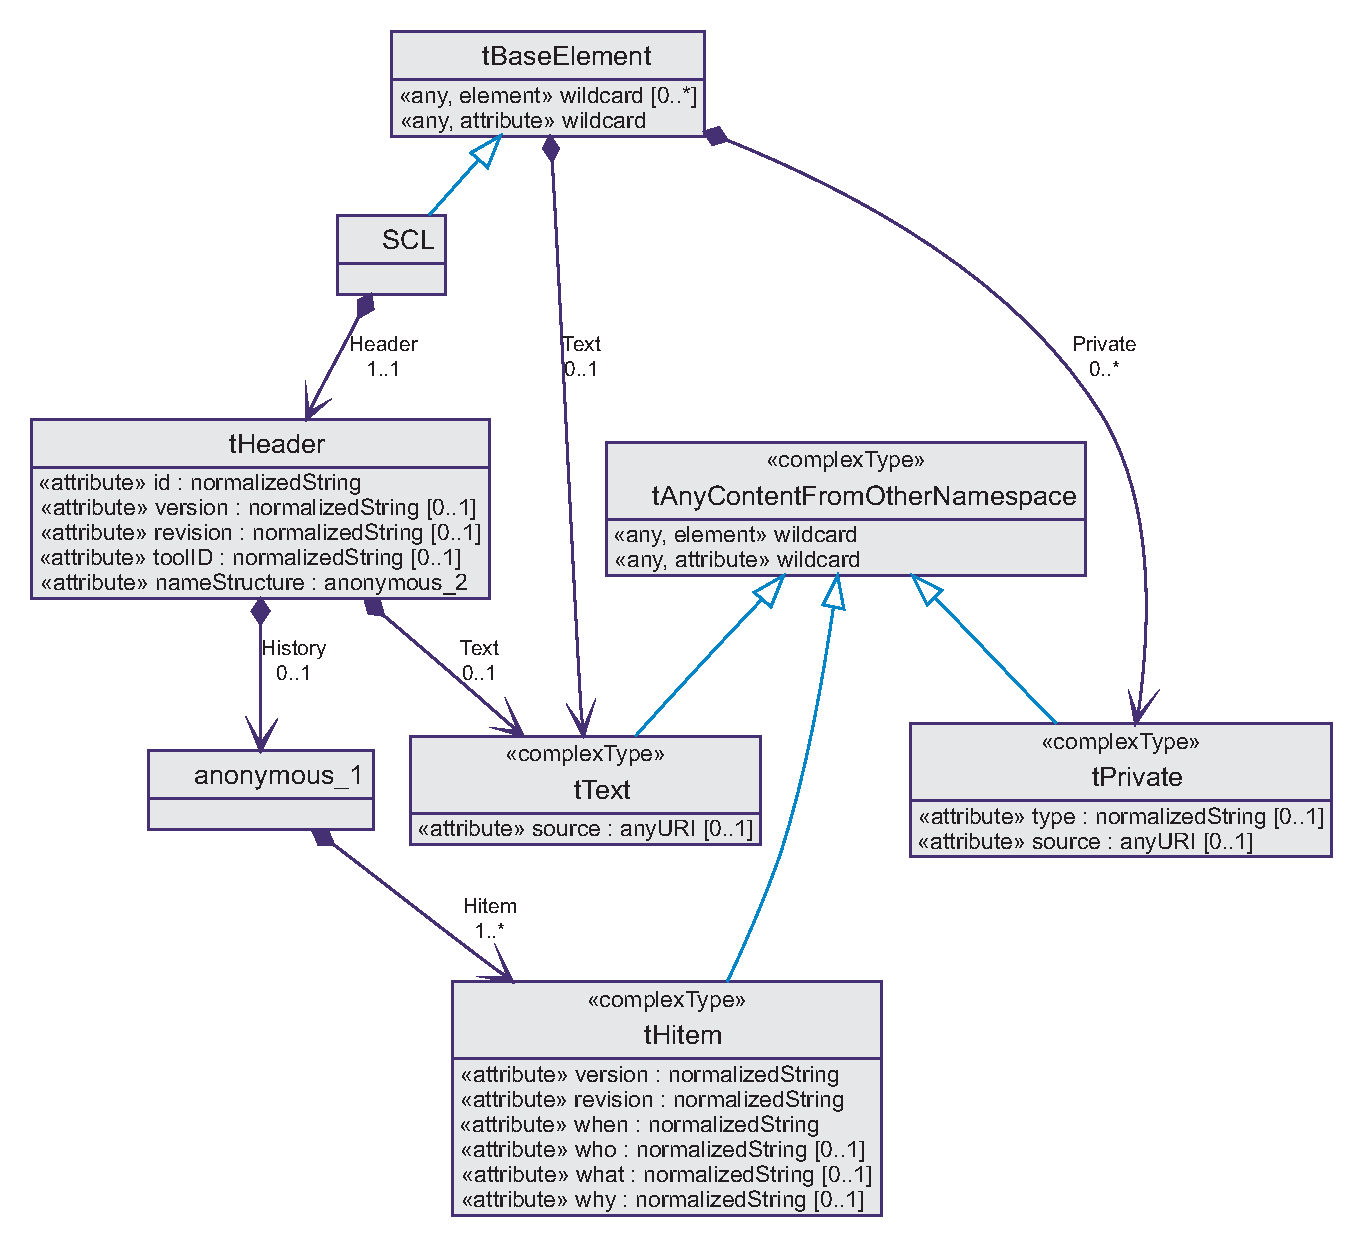
\includegraphics[width=1.0\textwidth]{chapters/enfoque/figures/scl-header-depthMax-conHerencia.eps}
  \caption{\emph{Header} del SCL, incluyendo las herencias
  correspondientes}
  \label{fig:SCL-header-con-herencias}
\end{center}
\end{figure}

El elemento \emph{Header} tambi�n define 
el enfoque del proceso de ingenier�a 
utilizado, pues con su atributo 
\emph{nameStructure} se indica 
si los nombres de se�ales del 
sistema de comunicaci�n proceden del 
elemento \emph{Substation} (generalmente
asociado con el archivo \gls{SSD}) 
o de la estructura de un IED existente 
en el mercado siendo sus posibles valores 
\emph{FuncName} o \emph{IEDName}. 

Con el enfoque utilizado en este trabajo 
se procede a la designaci�n de los nombres 
de las se�ales de comunicaci�n con 
respecto a los IEDs, pero no con IEDs 
procedentes del mercado, sino con 
ICDs dise�ados durante el proceso de ingenier�a
(en la secci�n \ref{chEnfoque:ied-simplif-no-preconfig} se proporciona 
m�s informaci�n sobre el 
enfoque utilizado en el
dise�o de los
modelos de IEDs realizados en este proyecto).

\begin{table}
	\lstinputlisting[label=cod:header-example-xml,
	caption=Ejemplo de Header]
	{chapters/enfoque/source/scl/myHeader.xml} 
\end{table}

Se provee de un trozo de ejemplo del 
ICD correspondiente a un IED a ser 
utilizado en la parte hidr�ulica 
del regualdor de velocidad en 
la lista \ref{cod:header-example-xml}. 
Esta estructura se visualiza mejor 
en el diagrama \gls{UML} 
de la figura \ref{fig:SCL-header-heredado}.  

\begin{figure}
\begin{center}
  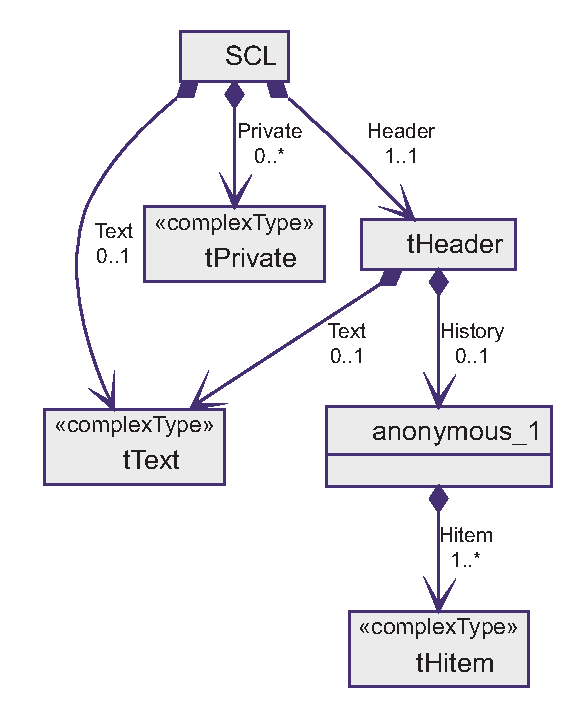
\includegraphics[width=0.4\textwidth]{chapters/enfoque/figures/scl-header-depthMax-heredado.eps}
  \caption{Clases instanciables del \emph{Header}}
  \label{fig:SCL-header-heredado}
\end{center}
\end{figure}





